\section{Results}
\label{sec:results}

\begin{table}[h]
\centering
\caption{Test-set results of the checkpoint with the best validation balanced accuracy ($n=\nTest$ images). Bal.\ acc.\ = balanced accuracy; min/ep.\ = mean training time per epoch on the laptop GPU.}
\label{tab:results}
\resizebox{\linewidth}{!}{%
\IfFileExists{results/results_table.tex}{\begin{tabular}{@{}lcccc@{}}
\toprule
Model & Test acc. & Test bal. acc. [95\% CI] & Macro F1 & min/ep. \\ \midrule
Majority (nv) & 0.676 & 0.143 & -- & -- \\
ResNet-50 & 0.773 & 0.706 [0.648, 0.764] & 0.607 & 3.2 \\
ViT-Base/16 & 0.745 & 0.728 [0.670, 0.784] & 0.610 & 8.2 \\
\bottomrule
\end{tabular}
}{\textit{Generated by train\_models.py.}}}
\end{table}

\begin{table}[h]
\centering
\caption{Per-class recall on the test set; $n$ is the number of test images per class.}
\label{tab:perclass}
\IfFileExists{results/per_class_recall.tex}{\begin{tabular}{@{}lccc@{}}
\toprule
Class & $n$ & ResNet-50 & ViT-Base/16 \\ \midrule
akiec & 34 & 0.765 & 0.765 \\
bcc & 89 & 0.820 & 0.674 \\
bkl & 168 & 0.500 & 0.583 \\
df & 9 & 0.556 & 0.667 \\
mel & 146 & 0.493 & 0.616 \\
nv & 974 & 0.856 & 0.793 \\
vasc & 21 & 0.952 & 1.000 \\
\bottomrule
\end{tabular}
}{\textit{Generated by train\_models.py.}}
\end{table}

Table~\ref{tab:results} summarises test performance.
ResNet-50 reaches a balanced accuracy of \resnetTestBacc{} \resnetTestBaccCI{} and accuracy \resnetTestAcc{}; ViT-Base reaches \vitTestBacc{} \vitTestBaccCI{} and \vitTestAcc{}.
The paired bootstrap difference in balanced accuracy (ResNet-50 minus ViT-Base) is \baccDiff{}, 95\% CI \baccDiffCI{}; if this interval contains zero, the run does not show a reliable difference between the two architectures.
Melanoma recall is \resnetMelRecall{} for ResNet-50 and \vitMelRecall{} for ViT-Base.
The best validation epoch was \resnetBestEpoch{} of \resnetEpochs{} for ResNet-50 and \vitBestEpoch{} of \vitEpochs{} for ViT-Base.
One training epoch took on average \resnetMinPerEpoch{} min for ResNet-50 and \vitMinPerEpoch{} min for ViT-Base.

% The numbers in this paragraph are from the 19 Nov 2026 run (results/*_metrics.json); update them if you rerun.
In balanced accuracy both models are far above the majority-class baseline, but in plain accuracy they are only 7--10 points above it: the class-weighted loss trades accuracy on the dominant nv class for recall on the rare classes.
Figure~\ref{fig:cm} shows where the errors are.
Melanoma is the main weakness of both models.
ViT-Base recalls more melanomas than ResNet-50 (90 vs.\ 72 of 146) but also labels about twice as many nevi as melanoma (143 vs.\ 72), so its melanoma precision is lower (0.34 vs.\ 0.42).
Many benign keratoses (bkl) are predicted as actinic keratoses (akiec), which gives akiec a low precision (0.25 and 0.33) despite a recall of 0.77 for both models.
Dermatofibroma (df) has only 9 test images, so its recall is not a reliable estimate.
Validation balanced accuracy at the selected epoch (0.722 and 0.750) is slightly higher than on the test set, as expected when the epoch is chosen on validation data.
Validation loss was still decreasing at epoch 5 for both models, so a longer schedule might help; this was not tested.

\begin{figure*}[t]
\centering
\IfFileExists{results/resnet50_confusion_test.png}{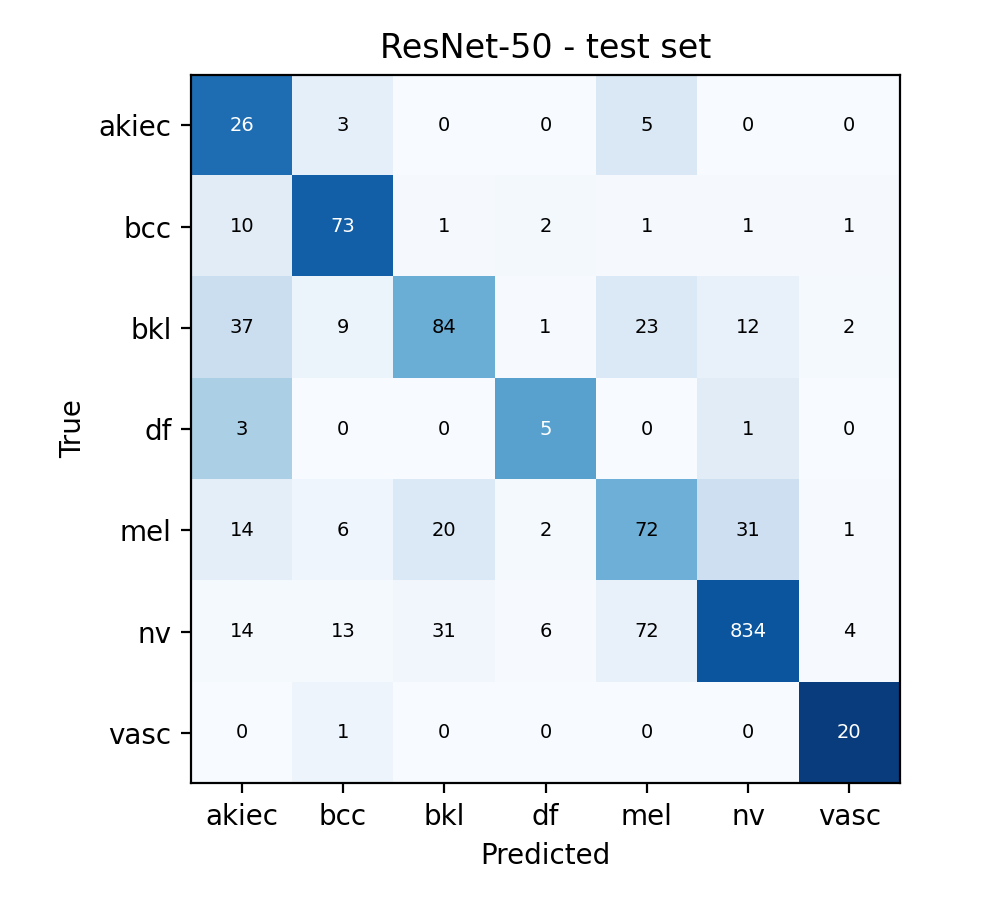
\includegraphics[width=0.42\textwidth]{results/resnet50_confusion_test.png}}{}%
\IfFileExists{results/vit_confusion_test.png}{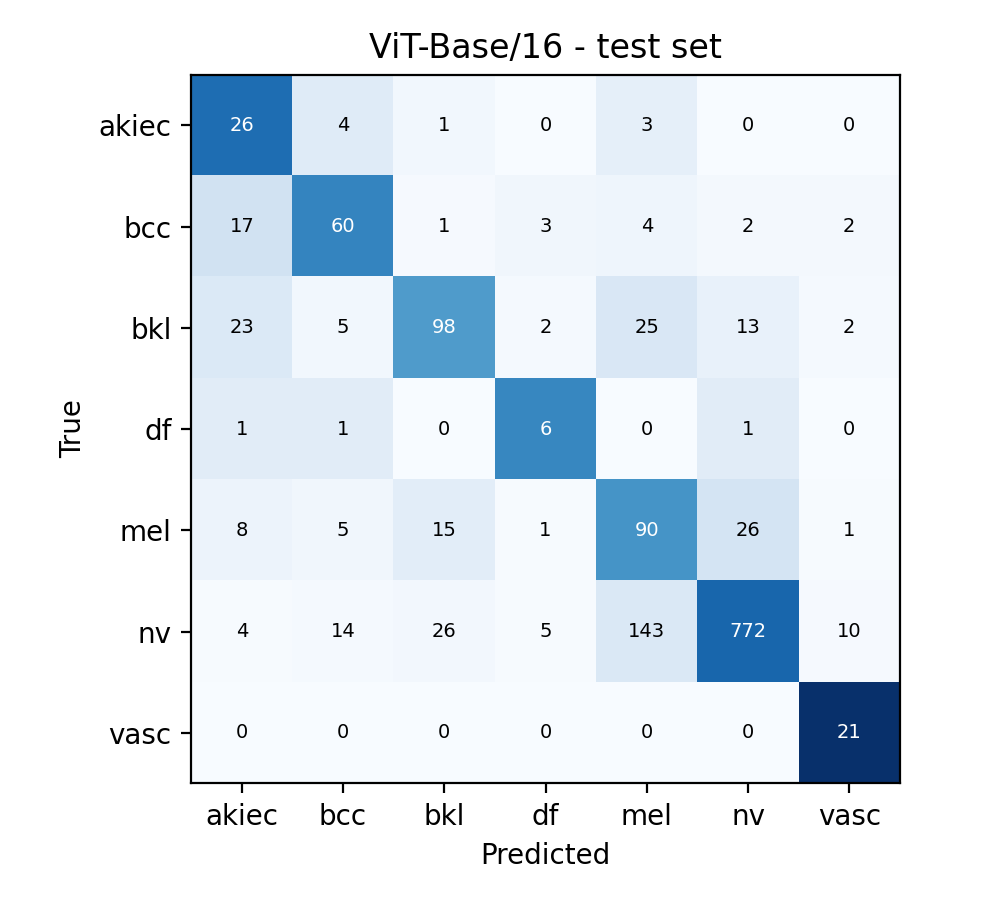
\includegraphics[width=0.42\textwidth]{results/vit_confusion_test.png}}{}
\caption{Test-set confusion matrices (counts; shading is row-normalised recall). Left: ResNet-50; right: ViT-Base.}
\label{fig:cm}
\end{figure*}
